%\documentclass[dvipsnames,handout, notes]{beamer}
\documentclass[dvipsnames]{beamer}
%%%%%%%%%%%%%Bibliography
\usepackage[backend=bibtex, url=false,
bibstyle=ieee,firstinits=true]{biblatex}
\renewcommand*{\thefootnote}{} %No symbol or marker
\renewcommand{\footnotesize}{\scriptsize}
%%%%%%%%%%%%%%%%%


\usepackage{xcolor}
\definecolor{chamois}{RGB}{255,255,240}
\definecolor{darkbrown}{RGB}{124,79,0}
\definecolor{UniBlue}{RGB}{83,101,130}

\definecolor{hellgelb}{rgb}{1,1,0.8}
\definecolor{colKeys}{rgb}{0,0,1}
\definecolor{colIdentifier}{rgb}{0,0,0}
\definecolor{colComments}{rgb}{1,0,0}
\definecolor{colString}{rgb}{0,0.5,0}

\usefonttheme{professionalfonts}
\usepackage{tgadventor}
\renewcommand*\familydefault{\sfdefault}
\usepackage[T1]{fontenc}
\usepackage{microtype}


\newcommand{\topline}{%
  \tikz[remember picture,overlay] {%
    \draw[brown,ultra thick] ([yshift=-1.8cm]current page.north west)-- ([yshift=-1.8cm,xshift=\paperwidth]current page.north west);} }

\renewcommand{\topline}{}

\setbeamertemplate{frametitle}{\begin{minipage}[b][1.8cm][c]{\textwidth}%
	\centering%
	\insertframetitle\\\insertframesubtitle
	\end{minipage}}
	

\addtobeamertemplate{frametitle}{}{\topline%
}

\setbeamertemplate{navigation symbols}{}
\setbeamercolor{background canvas}{bg=chamois}
\setbeamercolor{itemize item}{fg=brown}
%\setbeamertemplate{itemize item}{\maltese}
\setbeamercolor{itemize subitem}{fg=brown}
%\setbeamertemplate{itemize subitem}{\begin{rotate}{90}$\diamondsuit$\end{rotate}}

\setbeamercolor{title}{fg=UniBlue}
\setbeamercolor{frametitle}{fg=UniBlue}    
\setbeamerfont{frametitle}{size=\Large}

\setbeamercolor{author}{fg=darkbrown}
\setbeamercolor{institute}{fg=darkbrown}
\setbeamercolor{date}{fg=darkbrown}


\setbeamercolor{structure}{fg=UniBlue}
\setbeamercolor{alerted text}{fg=UniBlue}
\setbeamercolor{alerted text}{fg=UniBlue}
\setbeamercolor{normal text}{fg=darkbrown!50!black}
\setbeamercolor{math text}{fg=darkbrown}
\setbeamercolor{math text displayed}{fg=darkbrown}



\addtobeamertemplate{block begin}{%
	\setlength{\textwidth}{0.8\textwidth}%
}{}
\setbeamercolor{block title}{bg=darkbrown!40,fg=darkbrown!90}
\setbeamercolor{block body}{bg=darkbrown!20,fg=UniBlue}
\setbeamercolor{block title alerted}{bg=yellow!60,fg=red}
\setbeamercolor{block body alerted}{bg=hellgelb!80,fg=UniBlue}

\AtBeginSection[]{
	\begin{frame}
		\vfill
		\centering
		\begin{beamercolorbox}[sep=8pt,center,shadow=true,rounded=true]{title}
			\usebeamerfont{title}\insertsectionhead\par%
		\end{beamercolorbox}
		\vfill
	\end{frame}
}


% all notes should just be simple item notes.
% I neither need nor want more functionality
\let\oldnote\note
\renewcommand{\note}{\oldnote[item]}

%%%%%%%%%%%%%%%%%%%%%%%
% math
\usepackage{amsmath, amsthm, amssymb, mathtools}
\newcommand{\R}{\mathbb{R}}
\renewcommand{\v}{\varphi}
\newcommand{\vp}{\v^\prime}


\expandafter\def\expandafter\normalsize\expandafter{%
	\normalsize
	\setlength\abovedisplayskip{3pt}
	\setlength\belowdisplayskip{3pt}
	\setlength\abovedisplayshortskip{3pt}
	\setlength\belowdisplayshortskip{3pt}
}



%%%%%%%%%%%%%%%%%%%%%%%%%%%%%%%%%%%%%%%%%
% Graphics
\usepackage{graphicx}
\graphicspath{.}

\usepackage{tikz}
\usetikzlibrary{positioning}


\usepackage{pgfplots}
\pgfplotsset{compat=newest}
\pgfplotsset{
	every axis/.append style={
		width=1.15\textwidth,
		domain=-10:10,
		samples=101,
		smooth,
		no markers,
		ytick pos = left,
		xtick pos = left,
	}
}


%%%%%%%%%%%%%%%%%%%%%%%%%%%%%%%%
% ERF
\makeatletter
\pgfmathdeclarefunction{erf}{1}{%
	\begingroup
	\pgfmathparse{#1 > 0 ? 1 : -1}%
	\edef\sign{\pgfmathresult}%
	\pgfmathparse{abs(#1)}%
	\edef\x{\pgfmathresult}%
	\pgfmathparse{1/(1+0.3275911*\x)}%
	\edef\t{\pgfmathresult}%
	\pgfmathparse{%
		1 - (((((1.061405429*\t -1.453152027)*\t) + 1.421413741)*\t 
		-0.284496736)*\t + 0.254829592)*\t*exp(-(\x*\x))}%
	\edef\y{\pgfmathresult}%
	\pgfmathparse{(\sign)*\y}%
	\pgfmath@smuggleone\pgfmathresult%
	\endgroup
}
\makeatother
	
%%%%%%%%%%%%%%%%%%%%%%%%%%%%%%
\bibliography{master}
%%%%%%%%%%%%%%%%%%%%%%%%%%%%%

\author{\textbf{Lyndon White}, Chris Rackauckas (UCI)\\ Roberto Togneri, Wei Liu, Mohammed Bennamoun}
%\institute{School of Electical, Electronic and Computer Engineering\\The University of Western Australia}
\title{On the Properties of Neural Networks with Non-Negative Weights}
\subtitle{They are approximators for monotonic functions}


\begin{document}

\frame{\maketitle
	\note{
		So. Some observations on the properties of NNWNNs.
		They are Monotonic.
		Ok that is about it really.
		But actually though,	
		I'll begin by saying that I never intended to as come so close to Chris Bartley's stuff as I have.
		I didn't think these were general monotonic function approximators when I started playing with them.
		but they are.
		I do now get to cite Chris's work after the break as having proved some of the bits I need.
		So that is nice.
		And steal his motivating application area from a few years ago.
		I've not yet gotten to speak to him about this stuff directly.
	}
}

\begin{frame}{NNs and the Universal Approximation theorem}
	\vfill
	\begin{itemize}
		\item Neural networks are common machine learning systems
		\item They learn to approximate a function $\R^n \to \R^m$
		\item The function can be any continuous bounded function: that is the UAT \note{It is from several papers from the early 90s}
	\end{itemize}

	\vfill
	\citehere{mhaskar1992uat}\\
	\note{There is a new proof out this year by Sonoda, which to my knowledge is the first UAT proof in about a decade, that extends this. It was underreview for 2 years AFAICT. The math is really quiet scary.}
	\citehere{SONODA2017uat}
\end{frame}


\begin{frame}{NNs and the Universal Approximation theorem}
	\vfill
	\begin{itemize}
		\item It learns by adjusting neuron linking weight ($W$, $V$) and  activation basis ($\tilde{b}$, $\tilde{c}$).
		\item The UAT proofs don't actually tell us anyway to adjust those weights and biases.
		\item It just says that if you don't put any restrictions on them you can approximate anything.
	\end{itemize}
	\vfill
	
	\note{We generally just assume that gradient decent, based on showing some loss function derived from some training data set of example inputs an outputs works}
	\note{It normally does.}
	\centering
	\structure{\Large What if we did restrict the weights?}
\end{frame}


\begin{frame}{A single input single output neural network}
	\begin{block}{This is a SISO NN}
		\begin{align*}
			N(x;W,V,b,c) &= \sum_{j=1}^{j=n_h} V_{1,j} \v (b_j+W_{j,1}x_1) + c_1
		\end{align*}
	\end{block}

	\pause

	\begin{block}{This is its derivative}
		\begin{align*}
			\frac{\partial N(x;W,V,b,c)}{\partial x_1} = \sum_{j=1}^{j=n_h} V_{1,j}W_{j,1} \vp (b_j+W_{j,1}x_1)
		\end{align*}
	\end{block}
\end{frame}

\begin{frame}{A multi-input multi-output neural network}
	\begin{block}{This is a MIMO NN}
		\begin{align*}
	N(x;W,V,b,c)&=V\v(Wx+b)\\
	&=\left[\begin{array}{c}
{\displaystyle \sum_{j=1}^{j=n_{h}}}V_{1,j}\v\left(b_{j}+\sum_{i=1}^{i=n_{i}}\v\left(W_{j,i}x_{i}\right)\right) + c_1\\
\vdots\\
{\displaystyle \sum_{j=1}^{j=n_{h}}}V_{n_{o},j}\v\left(b_{j}+\sum_{i=1}^{i=n_{i}}\v\left(W_{j,i}x_{i}\right)\right) +c_{n_o}
\end{array}\right] \label{multiNNWNN}
		\end{align*}
	\end{block}
	
	\pause
	
	\begin{block}{This is its derivative (Jacobian)}
		\begin{align*}
		J_N&=\left(V\odot W^{T}\right)\vp(Wx+b)
		\end{align*}
	\end{block}
	\note{The Jacobian does not fit on the page when written in full. but it is basically a large matrix of elements that look like the SISO deritivite}
\end{frame}

\begin{frame}{How to make Weights Non-Negative}
	\begin{itemize}
		\item Some works use fancy contained optimisation, or regularisation-style penalties
		\item<2-> But much easier: just replace all the weights with some transforming function, whose output is nonnegative.
		\item<3-> Train it via backprop like usual
		\note{it is no issue with a autodiffing NN framework, and this is already an unconstrained nonlinear optimisation problem, so it doesn't in theory get anyharder.}
	\end{itemize}
	
	\begin{columns}[onlytextwidth]
		\begin{column}{0.33\textwidth}
			\centering
			\structure{Square} $w \mapsto w^2$
			\begin{tikzpicture}
			\begin{axis}[]
			\addplot {x^2};
			\end{axis}
			\end{tikzpicture}
		\end{column}
		
		
		\begin{column}{0.33\textwidth}
			\centering
			\structure{RELU} $w \mapsto max(0,w)$
			\begin{tikzpicture}
			\begin{axis}[]
			\addplot {max(0,x)};
			\end{axis}
			\end{tikzpicture}
		\end{column}
		
		
		\begin{column}{0.33\textwidth}
			\centering
			\structure{Exponentiate} $w\mapsto e^w$
			\begin{tikzpicture}
			\begin{axis}[scaled y ticks = false,  yticklabels={0, 0, 10K, 20K}]
			\addplot {exp(x)};
			\end{axis}
			\end{tikzpicture}
		\end{column}	
	\end{columns}	
\end{frame}

\def\cw{0.33\textwidth}

\newcommand{\actfuns}{
	\begin{columns}[onlytextwidth]
		\begin{column}{\cw}
			\centering
			\structure{Logistic}
			\begin{tikzpicture}
			\begin{axis}[]
			\addplot {1/(1+exp(-x))};
			\end{axis}
			\end{tikzpicture}
		\end{column}
		
		
		\begin{column}{\cw}
			\centering
			\structure{RELU6}
			\begin{tikzpicture}
			\begin{axis}[ytick={0,3,6}]
			\addplot {max(0,min(x,6))};
			\end{axis}
			\end{tikzpicture}
		\end{column}
		
		
		\begin{column}{\cw}
			\centering
			\structure{tanh}
			\begin{tikzpicture}
			\begin{axis}[]
			\addplot {tanh(x)};
			\end{axis}
			\end{tikzpicture}
		\end{column}
	
%		\begin{column}{\cw}
%			\centering
%			\structure{Normal Erf}
%			\begin{tikzpicture}
%			\begin{axis}[]
%			\addplot {0.5*(1+erf(x/sqrt(2)))};
%			\end{axis}
%			\end{tikzpicture}
%		\end{column}
	\end{columns}
}



\newcommand{\actfundiffs}{
	\begin{columns}[onlytextwidth]
		\begin{column}{\cw}
			\centering
			\structure{Logistic Sigmoid}
			\begin{tikzpicture}
			\begin{axis}[]
			\addplot {1/((1+exp(-x))*(1+exp(x)))};
			\end{axis}
			\end{tikzpicture}
		\end{column}
		
		
		\begin{column}{\cw}
			\centering
			\structure{RELU6}
			\begin{tikzpicture}
			\begin{axis}[]
			\addplot[domain=-10:0, blue,thick] {0};
			\addplot[domain=0:6, blue,thick] {1};
			\addplot[domain=6:10, blue,thick] {0};
			\end{axis}
			\end{tikzpicture}
		\end{column}
		
		
		\begin{column}{\cw}
			\centering
			\structure{tanh}
			\begin{tikzpicture}
			\begin{axis}[]
			\addplot {1-(tanh(x))^2};
			\end{axis}
			\end{tikzpicture}
		\end{column}	
	
%		\begin{column}{\cw}
%			\centering
%			\structure{Normal Erf}
%			\begin{tikzpicture}
%			\begin{axis}[]
%			\addplot {1/sqrt(2*pi) * exp(-0.5*x^2)};
%			\end{axis}
%			\end{tikzpicture}
%		\end{column}
	\end{columns}
}


\begin{frame}{This is a squashing activation function}
	\begin{block}<2->{$\v:\,\R \to \R$}
		\begin{itemize}
			\item monotonic
			\item bounded above and below
			\begin{itemize}
				\item WLOG assume by $0$,$1$
			\end{itemize}
			%\begin{align*}
			%\lim_{z\to-\infty} \v(z)=c_{min} \qquad \lim_{z\to\infty} \v(z)=c_{max}
			%\end{align*}
			\item differentiable almost everywhere \note{I might not have 100\% nailed down that regularity requirement yet}
		\end{itemize}
	\end{block}
	\vfill
	\actfuns{}
	
\end{frame}

\begin{frame}{This a squashing activation function's derivative, including the weight}
	\begin{block}<2->{$\dfrac{\partial\v(wx)}{\partial x}=w\vp(wx)$ \hfill It is a Summability Kernel}
		\begin{itemize}
			\item Uniformly continuous almost everywhere
			\item Non-negative, if $w$ is non-negative
			\item Finitely Integrable (i.e is $L^1$)
			\item $\forall \delta>0$, $\displaystyle\lim_{w->\infty} \int_{|x|>\delta} w\vp(wx) = 0$
			\note{It becomes more concentrated at the origin the smaller W is}
		\end{itemize}
		\note{These basically fall out of the FTC}
		
	\end{block}
	
	\actfundiffs{}
\end{frame}



\begin{frame}{A Summability Kernel is an Approximate Identity for Convolution}
	\begin{block}{What is convolution?}
		\note{You can relate convolution to convolutional neural networks, but that link is not relevant here}
		Convolution is an operation that takes two functions and gives a third.\\
		\begin{align*}
			f \ast g = \int_{-\infty}^\infty f(\tau)g(x-\tau) d\tau
		\end{align*}
		\note{It has applications in signal processing. Again, we don't care.}
	\end{block}
	
	\begin{block}<2->{Convolving with a summability kernal element does not change the function}
		For a function $f$ that is bounded and uniformly continuous.
		\begin{align*}
			\lim_{w\to\infty} f\ast\vp_w = f		\qquad \text{uniformly}
		\end{align*}
		
		\hfill (for $\vp_w(x)=w\vp(wx)$)
		\note{There are actually a bunch of different similar rules for different kinds of functions}
	\end{block}
\end{frame}

\section{Proof of Approximation Capacity}

\begin{frame}{Lets evaluate that convolution using a Reimann Sum}
	\begin{align*}
		f\ast\vp_W &= \int_{-\infty}^\infty f(x)\vp_w(x-\tau) d\tau\\
		&=\lim_{\Delta \to 0} \sum_{\forall i\in \mathbb{Z}} \Delta (f(i\Delta)\vp_w(x-i\Delta)) \qquad \text{uniformly}\\
	\end{align*}
	
	\note{Can probably only do this if it $f\ast\vp$ is compactly supported}
	
		

	\centering
	\begin{tikzpicture}
	\begin{axis}[width=0.9\textwidth,height=0.5\textheight, samples=15, bar width=1.5, yticklabels={}, xticklabels={}]
		\addplot[ybar, fill=blue]  {abs(0.00001*(x-7)*(4*x)*(x+11)*(x-100))^2};
		\addplot[samples=101, red, very thick] {abs(0.00001*(x-7)*(4*x)*(x+11)*(x-100))^2};
	\end{axis}
	\end{tikzpicture}

	
\end{frame}


\begin{frame}{What does that mean?}
	\begin{align*}
	f\ast\vp_W &= \int_{-\infty}^\infty f(x)\vp_w(x-\tau) d\tau\\
	&=\lim_{\Delta \to 0} \sum_{\forall i\in \mathbb{Z}} \bigg(\Delta (f(i\Delta)\bigg)w\vp(wx-i\Delta)) \quad \text{uniformly}
	\end{align*}
	
	\begin{block}<2->{i.e there exists values $\tilde{v}$, $\tilde{\beta}$ such that}
		\begin{align*}
		f\ast\vp_W &\approx \sum_{\forall (v_i,\beta_i)} v_i w\vp(wx-\beta_i))
		\end{align*}
	\end{block}
	\note{For an actually rigerous definition of approximately.}
	\note{and if $f$ is nonnegative, then so is $v$}
	\vfill
	{\footnotesize c.f. Lemma 2.2 of \citehere{bacharoglou2010approximation}.}
\end{frame}



\begin{frame}{Bring that together, with the Approximate Identity Property}
	\begin{block}{We have:}
	\begin{align*}
		f\ast\vp_w &\approx \sum_{\forall (v_i,\beta_i)} v_i w\vp(wx-\beta_i)) \\
		f\ast\vp_w &\approx f 
	\end{align*}
	\end{block}
	
	\begin{block}<2->{For any non-negative, compactly-supported continuous $f$ there exists values $w \ge 0$, $\tilde{v} \ge 0$, $\tilde{\beta}$ such that}
		\begin{align}
			f &\approx \sum_{\forall (v_i,\beta_i)} v_i w\vp(wx-\beta_i))
		\end{align}
	\end{block}
\end{frame}

\begin{frame}{Back to the NNWNN}
		\begin{align*}
			\frac{\partial N(x;W,V,b,c)}{\partial x_1} = \sum_{j=1}^{j=n_h} V_{1,j}W_{j,1} \vp (b_j+W_{j,1}x_1)
		\end{align*}
		\pause
		
		Choose $W_{j,1}=w$ and $V_{1,j}=v_i$ and $b_j=-\beta_i$.
		\note{We are actually throwing away some capacity here by restricting W to all be the same, but it turns out we never needed it anyway, as we still have full capacity}
		
		\pause
		
		\begin{align*}
		\frac{\partial N(x;W,V,b,c)}{\partial x_1} = \sum_{\forall (v_i,\beta_i)} v_i w\vp(wx-\beta_i) \approx f
		\end{align*}
		\pause
		\begin{block}{Integrate it all out and we get: $N(x;W,V,b,c)\approx F$}
			\note{have to do some fiddling to chose $c$}
			For $F$ being:
			\begin{itemize}
				\item Uniformly continuous a.e \note{(FTC)}
				\item Monotonic \note{(integral of nonnegative)}
				\item Bounded \note{(integral of compactly supported function)}
			\end{itemize}
			\note{We can throw in a bunch of almost everywheres because of various other densities of function spaces. But most are uninteresting}
		\end{block}
\end{frame}



\section{Proof of Approximation Lack of Capacity to do anything More}
\begin{frame}{It can only approximate monotonic bounded functions}
	\note{This one is easy}
	\begin{align*}
		N(x;W,V,b,c) &= \sum_{j=1}^{j=n_h} V_{1,j} \v (b_j+W_{j,1}x_1) + c_1
	\end{align*}
	\begin{itemize}
		\item It is the composition and sum of such functions.
		\item If $W$ and $V$ are non-negative.If $W$ and $V$ are non-negative.
		\item So it is also monotonic bounded \& continuous (a.e) functions
	\end{itemize}

	\note{Ignoring the almost everywhere part as it does not matter for approximation. As we used a $L^P$ based measure.}
	
	Such a function can not approximate a non-monotonic/bounded function as there would always be a difference.
\end{frame}


\section{What is it good for?}

\begin{frame}{Approximating Monotonic functions to make use of monotonic priors}

	\begin{itemize}
		\item This lets you incorporate expert knowledge
		\note{I told you I was going to steal Chris's intro}
		\note{All other factors being the same}
		\begin{itemize}
			\item The older the used-car the cheaper it is.
			\item The newer the computer the faster it runs.
			\item The newer the paper the better the performance on benchmarks.
		\end{itemize}
	\end{itemize}
	\note{This is useful as it increases user confidance in the system}
	\note{It decreases overfitting}
\end{frame}

\begin{frame}{Partially NNWNNs for partially monotonic functions.}
	\centering

	\vfill
	Consider two input network, with \alert{$x$ monotonic} and $z$ not.
	\vfill	
	\begin{tikzpicture}[x=25mm, y=18mm,
		nodes={draw=brownwrite,circle,minimum width=15mm},
		mono/.style={draw=bluewrite, text=bluewrite},
	]
	\node(out) at (0,0) {$N(x, z)$};
	\node(h1) at (.5,-1){};
	\node(h2) at (1.5,-1){};
	\node[mono](m1)  at (-.5,-1) {};
	\node[mono](m2)  at (-1.5,-1){};
	\node[mono](theta) at (-.75,-2) {$x$};
	\node(x) at (.75,-2) {$z$};
	\draw[mono, thick] (theta) -- (m1) -- (out) -- (m2) -- (theta);
	\draw[thick] (x) -- (h1) -- (out) -- (h2) -- (x);
	\draw[thick] (x) -- (m1);
	\draw[thick] (x) -- (m2);
	\end{tikzpicture}
	\vfill
	\alert{All weights on a path between output and monotonic input must be nonnegative.}
	\vfill
	\vfill
	\note{The brown half is for any fixed value of $z$ an normal NN}
	\note{The blue half is for any fixed value of $x$ an normal NNWNN}
	\note{Brown (normal) oututs can enter blue Monotonic nodes, but the reverse can not happen, or the network could learn a back-path to have a nonmonotic relation with $z$}
\end{frame}

\begin{frame}{All softmax classifiers can be NNWNNs}
	\begin{itemize}
		\item Monotonicity doesn't really factor into unordered categories
		\note{I am still working my head around what does it even mean to be monotonic in a multiclass classification setting.}
		\item A softmax output layer normalized the outputs of the layer below to sum to one.
		\note{The softmax basically sits on on top of the output layer of the NN (or NNWNN in this case)}
		\item so increasing one more than the other is the same as decreasing the others
		\item{so this is monotonic}
		\pause
		\item Note that this does not apply to single output classifier network \note{(e.g. binary choice / sigmoid)}
		\begin{itemize}
			\item Those can/will be made monotonic 
		\end{itemize}
	
	\end{itemize}
	
	\vfill
	{\footnotesize Proof in Appendix of \textcite{2014understandblenetworksnonnegweights}} 
\end{frame}

\section{Application In Continuous Probability Density Estimation}

\begin{frame}{We would like to estimate a PDF based on some observations}
	\centering		
	This is called non-parametric estimation.
	\note{There are many methods for doing this.}
	\note{There are many so called neural network methods for doing this}
	\note{Only a subset of those use normal enough structures that you can uses with as an LSTM as its input.}
	
	\vfill
	\includegraphics[width=0.9\textwidth]{gru256purplishgrey}\\
	Output from a color intention distribution estimation NN.\\
	3 separate softmax outputs on top of a GRU RNN
	\vfill
	Completely effective, but dissatisfying
	\vfill
	\note{This is the probability distribution for the color meant by Purplish Grey.}
	\note{This is from a prior project. It uses a 3 softmax layers with 256 bins to represent the colors possibly distributions}
	\note{It works great, and actually loses no information, as the original data is from monitors with only 8bits per channel}
	\note{It is highly distatistying though, to discretize the color space like this.}
	\note{Basically it irks me}
\end{frame}

\begin{frame}{Likas' 2001 neural PDF -- Using a normal NN}
	\begin{align*}
		f(x) \approx \dfrac{exp(N(x))}{\int_{\min(supp(f))}^{\max(supp(f))} exp(N(z)) dz}
	\end{align*}
	
	\begin{block}<2->{This is a PDF}
		\begin{itemize}
			\item Non-negative: via exponentiating
			\item Unit area: Divide out the area of the numerator.
		\end{itemize}
	\end{block}

	
	\begin{block}<3->{Problem: Slow.}
		\begin{itemize}
			\item You cannot integrate a neural network analytically.
			\item So use e.g. Gaussian Quadrature, every training batch.
		\end{itemize}
	\end{block}
	\vfill
	\citehere{likas2001probability}
\end{frame}

\begin{frame}{What if we differentiate it? So we know the integral}
	\note{I am tossing out the $exp$ as it doesn't do its purpose of nonnegative anymore.}
	\begin{block}{Neural Networks can be analytically differentiated}
		\begin{align*}
		f(x) &\approx \dfrac{N^\prime(x)}{N(\max(supp(f))) - N(\min(supp(f)))} \\
			 &\approx \dfrac{\sum_{j=1}^{j=n_h} V_{1,j}W_{j,1} \vp (b_j+W_{j,1}x_1)}{\sum_{k=1}^{k=n_h} \sum V_{1,k}}
		\end{align*}
	\end{block}
	\begin{block}<2->{This is not a PDF}
		\begin{itemize}
			\item Not non-negative \note{Even if we haven't thrown out the exp it wouldn't have helped}
			\item Yes, unit area: as before
		\end{itemize}
	\end{block}
	
	
	\begin{block}<2->{Unless W \& V are non-negative!}
		\begin{itemize}
			\item And now $N$ must be a NNWNN
		\end{itemize}
	\end{block}
\end{frame}

\begin{frame}{But look, it is actually a Almost GMM}
	\begin{block}{Look a but closer}
		\begin{align*}
		f(x) &\approx \dfrac{1}{\sum_{k=1}^{k=n_h} V_{1,k}} \sum_{j=1}^{j=n_h} V_{1,j}\, \bigg(W_{j,1} \vp (b_j+W_{j,1}x_1) \bigg)
		\end{align*}
	\end{block}
	\begin{block}<2->{ $f_j(x) = W_{j,1} \vp (b_j+W_{j,1}x_1)$}
		\begin{itemize}
			\item $f_j$ is a PDF
			\item $f$ is a thus mixture model
		\end{itemize}
	\end{block}
	
	\actfundiffs{}
	
	\note{This may or maynot be a particularly good parametric estimator}
	\note{It can outperform Lika,2001 on their own tests. But I'm not super happy with their methodology for testing.}
	\note{It is however a pretty normal neural network, compared to many (but not all) neural non-parametric estimators (E.g. generalised regression networks are not neural networks)}
	\note{This is good because}
\end{frame}

\begin{frame}{NNWNNs are Pretty Cool}
	\begin{itemize}
		\item They are just like normal neural networks except they must be monotonic.
		\item They can approximate bounded, and continuous any monotonic function.
		\item They can be useful for incorporating prior knowledge
		\item They can be useful for modelling CDFs
		\item It has been argued that they are more understandable -- less black-box

	\end{itemize}
\end{frame}


\end{document}